\chapter{Grundlagen}
\label{cha:Grundlagen}

\section{TDD}
\section{CI}
\section{SAP \& Mobile}

\subsection{SAP Gateway}
Das SAP Gateway wurde im Mai 2011 auf den Markt gebracht um die Reichweite von SAP-Geschäftsanwendungen zu erhöhen. 
Dazu bietet SAP mit dem Gateway eine offene REST-basierte Schnittstelle um einen einfachen Zugriff auf SAP-Systeme zu ermöglichen.
Das verwendete offene Protokoll OData wird dabei verwendet, da es viel genutzt, bekannt und leicht zu lernen ist. Damit soll die SAP-Welt jedem Entwickler geöffnet werden, der OData versteht, da kein spezielles SAP-Fachwissen mehr nötig ist um eine Oberfläche für Anwendungen zu entwickeln, die auf SAP-Daten zugreift.
Durch die Bereitstellung der OData-Schnittstelle müssen der Backend-Entwickler und der Frontend-Entwickler nicht wissen was der jeweils andere im Detail tut. Eine klare Definition der benötigten Schnittstellen allerdings zwingend notwendig und erleichtert die Entwicklung ungemein\cite[S.\ 31-45]{BoennenDreesFischerHeinzStrothmann2014}.

\begin{figure}[h]
\centering
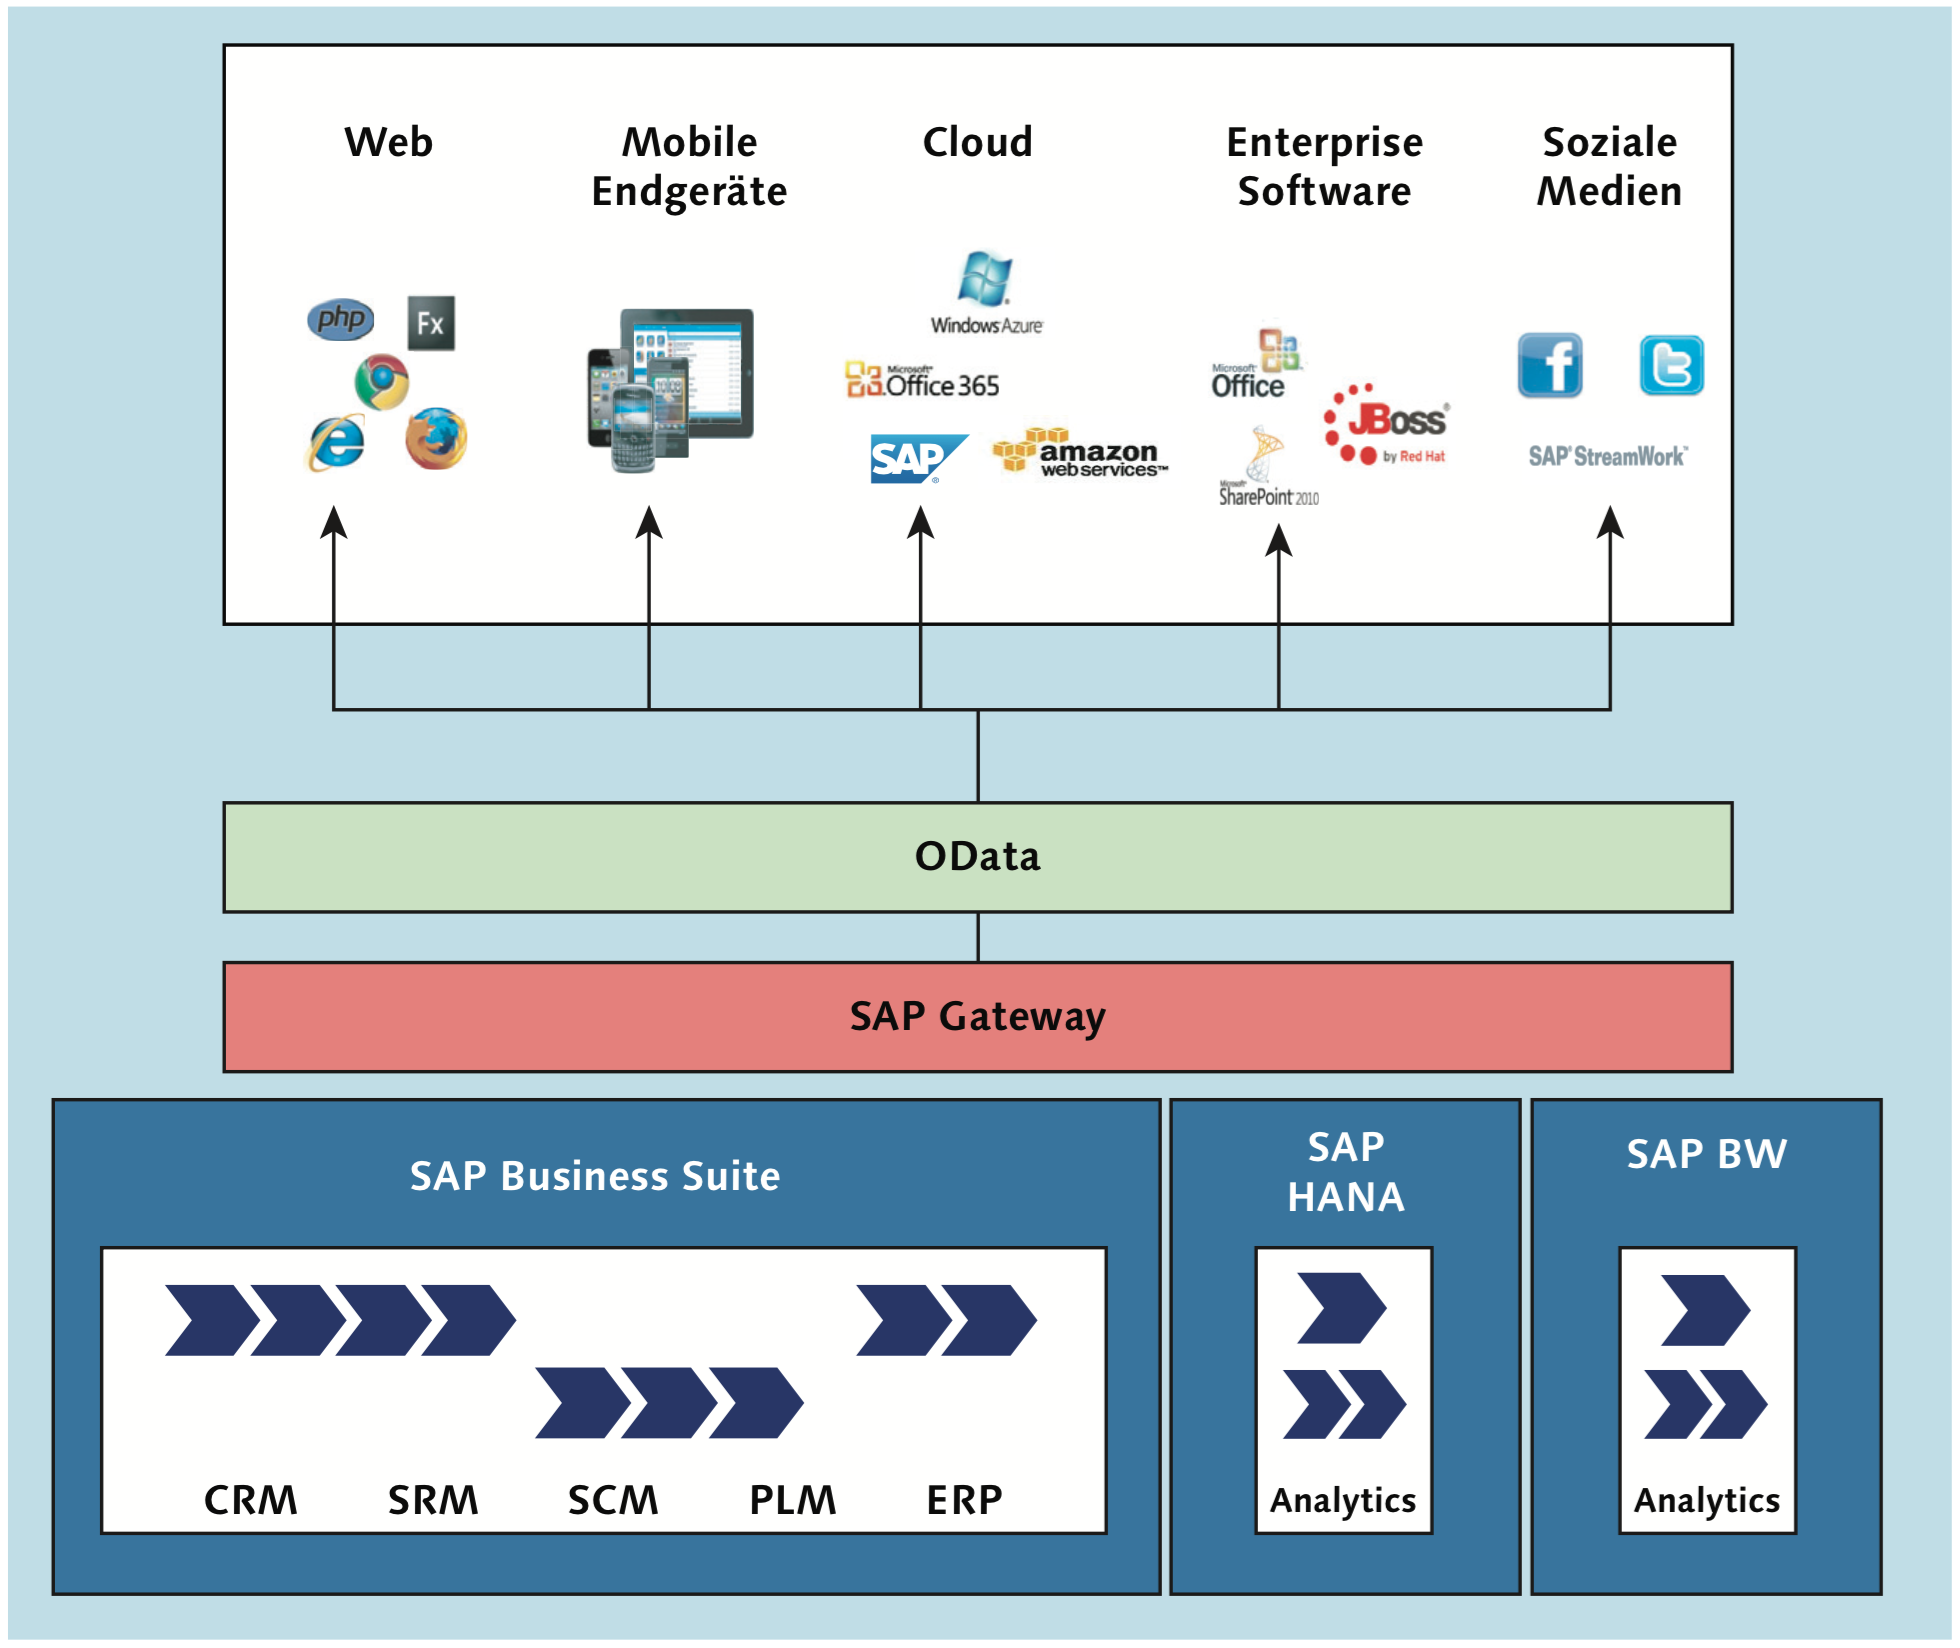
\includegraphics[width=.95\textwidth]{Gateway_architektur_page45} 
\caption{SAP Gateway- Schicht \cite[S.\ 45]{BoennenDreesFischerHeinzStrothmann2014}.}
\label{fig:CocaCola}
\end{figure}


\subsubsection{Deployment-Optionen}
Für das Deployment des SAP Gateway stehen verschiedene Optionen für das SAP Gateway welche im folgenden beschrieben werden.

\paragraph{eingebettetes Deployment}
Bei dieser Variante des Deployments werden alle Komponenten des SAP Gateways auf dem SAP Backend-System installiert. Der Hauptvorteil ist, dass die Laufzeit bei dieser Variante des Deployments um einen Remote Call reduziert wird, da der Service direkt auf dem Backend registriert wird. Der Nachteil an dieser Variante ist, dass das SAP Gateway für jedes Backend separat konfiguriert werden muss. Zudem rät SAP davon ab SAP-Backend-Systeme mit eingebettetem Gateway als Hub-System für andere SAP-Backend-Systeme zu verwenden, da mögliche Regeln zur Aktualisierung von System zu Fällen führen könnten in denen das  Hub-System nicht aktualisiert werden kann, obwohl das Backend-System bereits aktualisiert wurde\cite[S.\ 52-54]{BoennenDreesFischerHeinzStrothmann2014}.
 
\paragraph{Hub-Deployment mit Entwicklung auf dem SAP-Backend}
Hier werden die Gateway-Kernkomponenten auf einem zusätzlichem SAP Gateway Hub-System installiert. Zusätzlich muss auf dem SAP-Backend-System die Business-Enablement-Provisioning-Komponente \(IW\_BEP\) installiert werden. Bei dieser Variante wird auf dem Backend-System entwickelt und deployt und der Service wird anschließend auf dem Gateway Hub registriert. Beim Hub-Deployment ist es möglich mehrere SAP Backend-Systeme mit dem Gateway zu verbinden. 
Zudem gibt es hier keinen direkten Zugriff auf das SAP Backend-System\cite[S.\ 54]{BoennenDreesFischerHeinzStrothmann2014}.

\paragraph{Hub-Deployment mit Entwicklung auf dem Hub}
Hier werden alle Komponenten des SAP Gateways auf dem Hub-System installiert. Diese Variante wird zum Beispiel eingesetzt wenn der Zugriff auf das Backend-System eingeschränkt und eine Entwicklung auf diesem nicht möglich ist oder bei Releaseständen unter SAP NetWeaver 7.40, da eine Installation von IW\_BEP nicht erlaubt ist. Die Entwicklung des Services findet auf dem Hub-System statt. Der Vorrteil ist, dass das SAP Backend-System nicht angefasst werden muss. Allerdings muss bei der Entwicklung auf Funktionalitäten wie z.B. RFCs oder BAPIs zurückgegriffen werden, die vom Backend bereitgestellt werden müssen\cite[S.\ 55]{BoennenDreesFischerHeinzStrothmann2014}.


 %http://scn.sap.com/community/gateway/blog/2013/05/27/sap-netweaver-gateway-deployment-options-in-a-nutshell

%Vor NW 7.40 -> Installieren von GW_CORE, IW_FND, IW_BEP 